\documentclass[tikz,border=12pt]{standalone}
\usepackage[T1]{fontenc}
\usepackage{mathpazo}
\usepackage{amsmath,amssymb}
\usetikzlibrary{arrows.meta, calc, positioning}

\definecolor{stblue}{HTML}{7B97AD}
\definecolor{rwgold}{HTML}{B8995E}
\definecolor{sage}{HTML}{7A9A7E}
\definecolor{dkbrown}{HTML}{3D3530}
\definecolor{wmgray}{HTML}{7B7067}
\definecolor{cream}{HTML}{F9F6F0}
\definecolor{border}{HTML}{D4C9B8}
\definecolor{terracotta}{HTML}{C47A6A}
\definecolor{lavender}{HTML}{907EA0}

\begin{document}
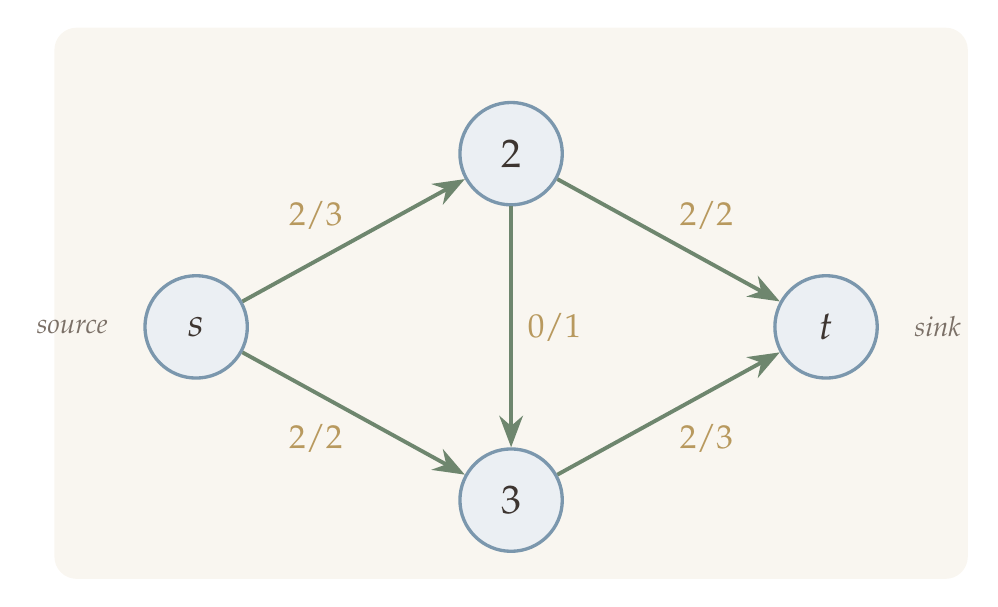
\begin{tikzpicture}[
    >={Stealth[length=4mm, width=3mm]},
    every node/.style={text=dkbrown},
  ]

  % Background
  \fill[cream, rounded corners=8pt] (-1.8,-3.2) rectangle (9.8,3.8);

  % Nodes
  \node[circle, fill=stblue!15, draw=stblue, line width=1.2pt,
        minimum size=1.3cm, font=\Large\bfseries] (1) at (0,0) {$s$};
  \node[circle, fill=stblue!15, draw=stblue, line width=1.2pt,
        minimum size=1.3cm, font=\Large] (2) at (4,2.2) {$2$};
  \node[circle, fill=stblue!15, draw=stblue, line width=1.2pt,
        minimum size=1.3cm, font=\Large] (3) at (4,-2.2) {$3$};
  \node[circle, fill=stblue!15, draw=stblue, line width=1.2pt,
        minimum size=1.3cm, font=\Large\bfseries] (4) at (8,0) {$t$};

  % Edge style
  \tikzset{
    flowedge/.style={->, line width=1.4pt, sage!80!dkbrown},
  }

  % Edge 1 -> 2 (flow 2, capacity 3)
  \draw[flowedge] (1) -- (2)
    node[midway, above left, font=\large] {%
      \textcolor{rwgold}{2/3}};

  % Edge 1 -> 3 (flow 2, capacity 2)
  \draw[flowedge] (1) -- (3)
    node[midway, below left, font=\large] {%
      \textcolor{rwgold}{2/2}};

  % Edge 2 -> 3 (flow 0, capacity 1)
  \draw[flowedge] (2) -- (3)
    node[midway, right=2pt, font=\large] {%
      \textcolor{rwgold}{0/1}};

  % Edge 2 -> 4 (flow 2, capacity 2)
  \draw[flowedge] (2) -- (4)
    node[midway, above right, font=\large] {%
      \textcolor{rwgold}{2/2}};

  % Edge 3 -> 4 (flow 2, capacity 3)
  \draw[flowedge] (3) -- (4)
    node[midway, below right, font=\large] {%
      \textcolor{rwgold}{2/3}};

  % Source / sink labels
  \node[font=\normalsize\itshape, text=wmgray, anchor=east] at (-1.0,0) {source};
  \node[font=\normalsize\itshape, text=wmgray, anchor=west] at (9.0,0) {sink};

\end{tikzpicture}
\end{document}
